\let\negmedspace\undefined
\let\negthickspace\undefined
\documentclass[journal,12pt,twocolumn]{IEEEtran}
\usepackage{gensymb}
\usepackage{amssymb}
\usepackage[cmex10]{amsmath}
\usepackage{amsthm}
\usepackage[export]{adjustbox}
\usepackage{bm}
\usepackage{longtable}
\usepackage{enumitem}
\usepackage{mathtools}
\usepackage[breaklinks=true]{hyperref}
\usepackage{listings}
\usepackage{color}                                            %%
\usepackage{array}                                            %%
\usepackage{longtable}                                        %%
\usepackage{calc}                                             %%
\usepackage{multirow}                                         %%
\usepackage{hhline}                                           %%
\usepackage{ifthen}                                           %%
\usepackage{lscape}     
\usepackage{multicol}
\documentclass{amsart}
% \usepackage{enumerate}
\DeclareMathOperator*{\Res}{Res}
\renewcommand\thesection{\arabic{section}}
\renewcommand\thesubsection{\thesection.\arabic{subsection}}
\renewcommand\thesubsubsection{\thesubsection.\arabic{subsubsection}}
\renewcommand\thesectiondis{\arabic{section}}
\renewcommand\thesubsectiondis{\thesectiondis.\arabic{subsection}}
\renewcommand\thesubsubsectiondis{\thesubsectiondis.\arabic{subsubsection}}
\hyphenation{op-tical net-works semi-conduc-tor}
\def\inputGnumericTable{}                                 %%

\lstset{
frame=single, 
breaklines=true,
columns=fullflexible
}
\begin{document}
\newtheorem{theorem}{Theorem}[section]
\newtheorem{problem}{Problem}
\newtheorem{proposition}{Proposition}[section]
\newtheorem{lemma}{Lemma}[section]
\newtheorem{corollary}[theorem]{Corollary}
\newtheorem{example}{Example}[section]
\newtheorem{definition}[problem]{Definition}
\newcommand{\BEQA}{\begin{eqnarray}}
\newcommand{\EEQA}{\end{eqnarray}}
\newcommand{\define}{\stackrel{\triangle}{=}}
\bibliographystyle{IEEEtran}
\providecommand{\mbf}{\mathbf}
\providecommand{\pr}[1]{\ensuremath{\Pr\left(#1\right)}}
\providecommand{\qfunc}[1]{\ensuremath{Q\left(#1\right)}}
\providecommand{\sbrak}[1]{\ensuremath{{}\left[#1\right]}}
\providecommand{\lsbrak}[1]{\ensuremath{{}\left[#1\right.}}
\providecommand{\rsbrak}[1]{\ensuremath{{}\left.#1\right]}}
\providecommand{\brak}[1]{\ensuremath{\left(#1\right)}}
\providecommand{\lbrak}[1]{\ensuremath{\left(#1\right.}}
\providecommand{\rbrak}[1]{\ensuremath{\left.#1\right)}}
\providecommand{\cbrak}[1]{\ensuremath{\left\{#1\right\}}}
\providecommand{\lcbrak}[1]{\ensuremath{\left\{#1\right.}}
\providecommand{\rcbrak}[1]{\ensuremath{\left.#1\right\}}}
\theoremstyle{remark}
\newtheorem{rem}{Remark}
\newcommand{\sgn}{\mathop{\mathrm{sgn}}}
\providecommand{\abs}[1]{\left\vert#1\right\vert}
\providecommand{\res}[1]{\Res\displaylimits_{#1}} 
\providecommand{\norm}[1]{\left\lVert#1\right\rVert}
%\providecommand{\norm}[1]{\lVert#1\rVert}
\providecommand{\mtx}[1]{\mathbf{#1}}
\providecommand{\mean}[1]{E\left[ #1 \right]}
\providecommand{\fourier}{\overset{\mathcal{F}}{ \rightleftharpoons}}
%\providecommand{\hilbert}{\overset{\mathcal{H}}{ \rightleftharpoons}}
\providecommand{\system}{\overset{\mathcal{H}}{ \longleftrightarrow}}
	%\newcommand{\solution}[2]{\textbf{Solution:}{#1}}
\newcommand{\solution}{\noindent \textbf{Solution: }}
\newcommand{\cosec}{\,\text{cosec}\,}
\providecommand{\dec}[2]{\ensuremath{\overset{#1}{\underset{#2}{\gtrless}}}}
\newcommand{\myvec}[1]{\ensuremath{\begin{pmatrix}#1\end{pmatrix}}}
\newcommand{\mydet}[1]{\ensuremath{\begin{vmatrix}#1\end{vmatrix}}}
\numberwithin{equation}{subsection}
\makeatletter
\@addtoreset{figure}{problem}
\makeatother
\let\StandardTheFigure\thefigure
\let\vec\mathbf
\renewcommand{\thefigure}{\theproblem}
\def\putbox#1#2#3{\makebox[0in][l]{\makebox[#1][l]{}\raisebox{\baselineskip}[0in][0in]{\raisebox{#2}[0in][0in]{#3}}}}
     \def\rightbox#1{\makebox[0in][r]{#1}}
     \def\centbox#1{\makebox[0in]{#1}}
     \def\topbox#1{\raisebox{-\baselineskip}[0in][0in]{#1}}
     \def\midbox#1{\raisebox{-0.5\baselineskip}[0in][0in]{#1}}
\vspace{3cm}
\title{
	10th CBSE MATHEMATICS
}
\author{ 2012-13
	\thanks{}
	
}
\maketitle
\newpage
\bigskip
\renewcommand{\thefigure}{\theenumi}
\renewcommand{\thetable}{\theenumi}
\end{abstract}
\section{Section A}
\renewcommand{\theequation}{\theenumi}
\begin{enumerate}[label=\thesection.\arabic*.,ref=\thesection.\theenumi]
\numberwithin{equation}{enumi}
\item The roots of the  quadratic equation $2x^2-x-6=0$ are :
 \begin{enumerate}[A]
    \item -2,3/2\\
    \item 2, -3/2\\
    \item -2, 3/2\\
    \item 2, 3/2\\
 \end{enumerate} 
\item If the  $n^{\text{th}}$ term of an A.P. is (2n+ 1), then the sum of its first three terms is
 \begin{enumerate}[A]
    \item $6n + 3$\\
    \item 15 \\
    \item 12\\
    \item 21 \\
 \end{enumerate}
\item From a point Q, 13 cm away from the centre of a circle, the length of tangent PQ to the circle is 12 cm. The radius of the circle (in cm)
is \\
 \begin{enumerate}[A]
    \item 25\\
    \item $\sqrt{313}$\\
    \item 5\\
    \item 1 \\
 \end{enumerate}
\item In Fig. \ref{fig1}, 1, AP, AQ and BC are tangents of the circle. If AB = 5cm, AC = 6cm and BC = 4 cm, then the length of AP (in cm) is \\
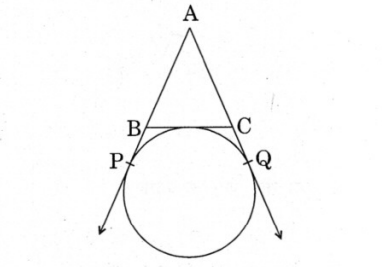
\includegraphics[width=0.5\columnwidth,center]{1.png}\\{\centering
\caption{Fig. 1}\\}
\label{fig1}
 \begin{enumerate}[A]
    \item $7.5$\\
    \item 15 \\
    \item 10 \\
    \item 9
 \end{enumerate}
\item The circumference of a circle is 22 cm. The area of its quadrant (in $cm^2$) is
 \begin{enumerate}[A]
    \item $\frac{77}{2}$\\
    \item $\frac{77}{4}$\\
    \item $\frac{77}{8}$\\
    \item $\frac{77}{16}$\\
 \end{enumerate}
 \item A solid right circular cone is cut into two parts at the middle of its height by a plane parallel to its base. The radio of the volume of the smaller cone to the whole cone is
 \begin{enumerate}[A]
    \item 1:2 \\
    \item 1:4 \\ 
    \item 1:6 \\
    \item 1:8 \\
 \end{enumerate}
\item A kite is flying at a height of 30 m from the ground. The length of string from the kite to the ground is 60 m. Assuming that there is no slack in the string, the angle of elevation of the kite at the ground is
\begin{enumerate}[A]
    \item $45\degree$\\
    \item $30\degree$\\
    \item $60\degree$\\
    \item $90\degree$\\
 \end{enumerate}
\item The distance of the point $(-3 , 4)$ from the x-axis is
 \begin{enumerate}[A]
    \item 3\\
    \item -3\\
    \item 4\\
    \item 5 \\
 \end{enumerate}
\item In Fig. \ref{fig2}, $P(5, -3)$ and $Q(3, y)$ are the points of trisection of the line segment joining $A(7, -2)$ and $B(1, -5)$. Then y equals.\\

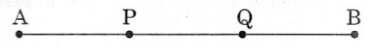
\includegraphics[width=0.5\columnwidth,center]{2.png}\\{\centering
\caption{Fig. 2}\\}
\label{fig2}
 \begin{enumerate}[A]
  \item 2\\
  \item 4 \\
  \item -4 \\
  \item $-\frac{5}{2}$
\end{enumerate}
\item Cards bearing numbers 2,3,4, ..., 11 are kept in a bag. A card is drawn at random from the bag. The probability of getting a card with a prime number is\\
 \begin{enumerate}
     \item $\frac{1}{2}$\\
     \item $\frac{2}{5}$\\
     \item $\frac{3}{10}$\\
     \item $\frac{5}{9}$\\
 \end{enumerate}
 \end{enumerate}
\section{Section B}
\renewcommand{\theequation}{\theenumi}
\begin{enumerate}[label=\thesection.\arabic*.,ref=\thesection.\theenumi]
\numberwithin{equation}{enumi}
\item Find the value of p for which the roots of the equation $px(x-2+6=0$, are equal.\\
\item How many two-digit natural numbers are divisible by 3?\\
\item In Fig. \ref{fig3}, a right triangle ABC, circumscribes a circle of radius r. If AB and BC are of lengths 8cm and 6cm respectively, find the value of r. \\

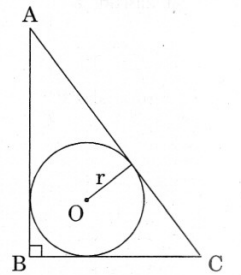
\includegraphics[width=0.5\columnwidth,center]{3.png}\\{\centering
\caption{Fig. 3}\\}
\label{fig3}\\
\item Prove that the tangents drawn at the ends of a diameter of a circle are parallel.\\
\item In Fig. \ref{fig4}, ABCD is a square of side 4 cm. A quadrant of a circle of radius 1 cm in drawn at each vertex of the square and a circle of diameter 2 cm is also drawn. Find the area of the shaded region. (Use $\pi = 3.14)$\\

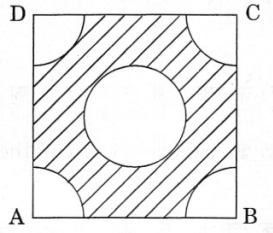
\includegraphics[width=0.5\columnwidth,center]{4.png}\\{\centering
\caption{Fig. 4}\\}
\label{fig4}\\
\begin{center}
    \bold{OR}
\end{center}
From a rectangular sheet of paper ABCD with AB = 40 cm and AD = 28 cm, a semi-circular portion with BC as diameter is cut off. Find the area of the remaining paper. (Use $\pi=\frac{22}{7}$)\\
\item A solid sphere of radius 10.5 cm is melted and recast into smaller solid cones, each of radius 3.5 cm and height 3 cm. Find the number of cones so formed. (Use $\pi=\frac{22}{7}$)\\
\item Find the value of k, if the point $P(2, 4)$ is equidistant from the points $A(5, k)$ and $B(k, 7)$.
\item A card is drawn at random from a well-shuffled pack of 52 cards. Find the
probability of getting\\
 \begin{enumerate}
     \item a red king
     \item a queen or a jack\\
 \end{enumerate}
\section{Section C}
\renewcommand{\theequation}{\theenumi}
\begin{enumerate}[label=\thesection.\arabic*.,ref=\thesection.\theenumi]
\numberwithin{equation}{enumi}
\item Solve the following quadratic equation for x: \\
$x^2-4ax-b^2+4a^2=0$\\
\item Find the sum of all multiples of 7 lying between 500 and 900. \\
\item Draw a triangle ABC with $BC = 7cm$, $\angle B = 45\degree$ and $\angle C = 60\degree$. Then construct another triangle, whose sides are times the corresponding sides of  $\triangle ABC.$ \\
\item In Fig. \ref{fig5}, a circle is inscribed in a triangle PQR with PQ = 10cm, QR = 8cm and PR = 12cm. Find the lengths QM, RN and PL.\\

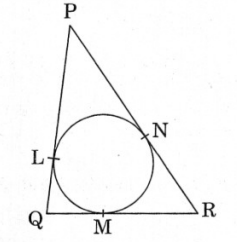
\includegraphics[width=0.5\columnwidth,center]{5.png}\\
{\centering
\caption{Fig. 5}\\}
\label{fig5}
\item In Fig. \ref{fig6}, is the centre of the circle with $AC = 24cm$, $AB=7cm$ and $\angle BOD = 90\degree$. Find the area of the shaded region. (Use $\pi = 3.14$)\\

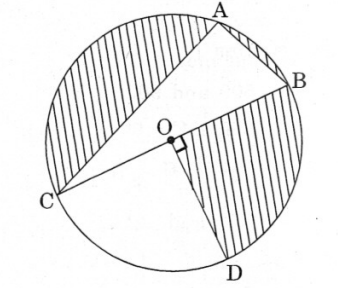
\includegraphics[width=0.5\columnwidth,center]{6.png}\\{\centering
\caption{Fig. 6}\\}
\label{fig6}\\
\begin{center}
    \bold{OR}
\end{center}
In Fig. \ref{fig7}, find the area of the shaded region, if ABCD is a square of side 14 cm and APD and BPC are semicircles.\\

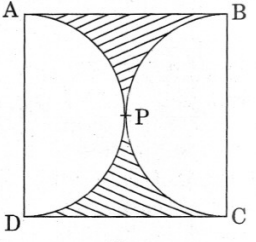
\includegraphics[width=0.5\columnwidth,center]{7.png}\\{\centering
\caption{Fig. 7}\\}
\label{fig7}\\
\item A hemispherical bowl of internal radius 9 cm is full of water. Its contents are emptied in a cylindrical vessel of internal radius 6 cm. Find the height of water in the cylindrical vessel.\\
\item The angles of depression of the top and bottom of a tower as seen from the top of a 60 $\sqrt{3}$ m high cliff are $45\degree$ and $60\degree$ respectively. Find the height of the tower.\\
\item Find the coordinates of a point P, which lies on the line segment joining the points $A(-2, -2)$ and $B(2, -4)$ such that \\ $AP =\frac{3}{7} \ AB$.
\begin{center}
    \bold{OR}
\end{center}
Find the area of the quadrilateral ABCD whose vertices are
$A(-3, -1)$, $B(-2, -4)$, $C(4, - 1)$ and $D(3, 4)$.\\
\item All kings, queens and aces are removed from a pack of 52 cards. The remaining cards are well shuffled and then a card is drawn from it. Find the probability that the drawn card is
 \begin{enumerate}[A]
    \item a black face card
    \item a red card\\
 \end{enumerate}
\item The numerator of a fraction is 3 less than its denominator. If 1 is added to the denominator, the fraction is decreased by $\frac{1}{15}$ Find the fraction.
\begin{center}
    \bold{OR}
\end{center}
In a flight of 2800 km, an aircraft was slowed down due to bad
weather. Its average speed is reduced by 100 km/h and time
increased by 30 minutes. Find the original duration of the flight.\\
\item Find the common difference of an A.P. whose first term is 5 and the sum of its first four terms 1s half the sum of the next four terms.\\
\item Prove that the length of tangents drawn from an external point to a circle are equal.\\
\item A hemispherical tank, full of water, is emptied by a pipe at the rate of $\frac{25}{7}$ litres per sec. How much time will it take to empty half the tank if the diameter of the base of the tank is 3m?\\
\begin{center}
\bold{OR}
\end{center}
A drinking glass is in the shape of the frustum of a cone of height 14cm. The diameters of its two circular ends are 4cm and 2cm. Find the capacity of the glass. (Use $\pi = \frac{22}{7}$)\\
\item A military tent of height 8:25 m is in the form of a right circular cylinder of base diameter 30 m and height 5.5 m surmounted by a right circular cone of same base radius. Find the length of the canvas use in making the tent, if the breadth of the canvas is 1.5m.\\
\item The angles of elevation and depression of the top and bottom of a light-house from the top of a 60 m high building are 30 and 60 respectively. Find
 \begin{enumerate}[A]
  \item the difference between the heights of the light-house and the building.
  \item the distance between the light-house and the building
 \end{enumerate}
\end{enumerate} 
\end{enumerate}
\end{enumerate}
\end{document}
